\chapter{Introduzione alle reti neurali}

Le reti neurali, grazie alla loro capacità di gestire dati non lineari e molto rumorosi, e di riconoscere pattern complessi, ritrovano moltissime applicazioni per la risoluzione di task di vario tipo. Esistono inoltre numerose varianti delle reti neurali (profonde e non), tra cui la MLP (di cui parleremo) e la CNN.


\section{Definizione di rete neurale}

\begin{figure}[htbp]
	\centering
	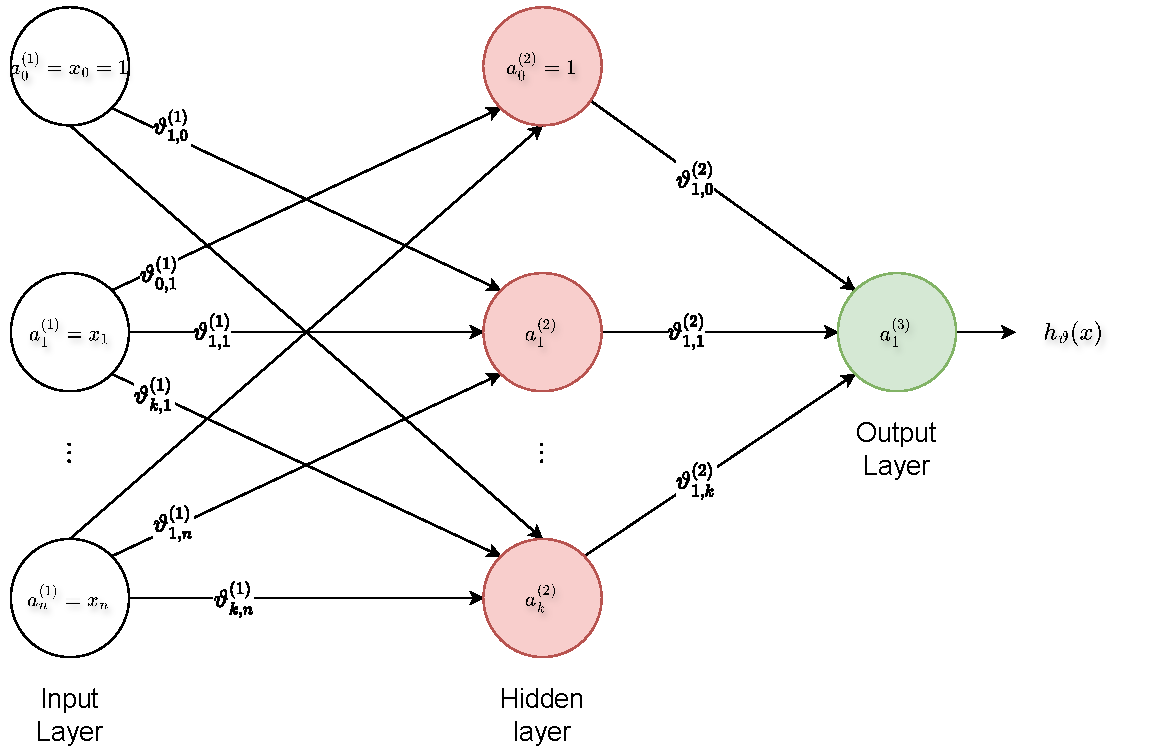
\includegraphics[width=0.8\linewidth]{images/NeuralNet1pdf}
	\caption{Un multilayer perceptron, ossia una particolare rete neurale.}
	\label{fig:mlp_nn}
\end{figure}

Una rete neurale è una funzione matematica \textit{annidata} del tipo:

$$
f_n(f_{n-1}(\dots (f_1(x))))
$$

dove $n$ coincide col numero di strati, o \textit{layer}. Questa rete neurale ritorna uno scalare $y$.  Una rete neurale è quindi ottenuta da una \textbf{composizione di funzioni derivabili}. Le funzioni sono dette \textbf{funzioni di attivazione}, e andremo a vederne presto alcuni esempi. Ogni funzione $f_i$ è detta \textbf{layer} che è composto da un certo numero di \textbf{neuroni}, o unità, che sono a loro volta composti da:
\begin{itemize}
	\item Una trasformazione lineare $z = W x + b$, in cui $W$ è la matrice dei pesi, $b$ è il bias, e $x$ è l'input del layer. Il numero di neuroni di un layer determina il numero di righe della matrice dei pesi $W$.
	\item Una funzione di attivazione $a = \sigma(z)$, che introduce non linearità nella rete. La funzione di attivazione viene applicata elemento per elemento al vettore $z$.
\end{itemize}

I neuroni di un layer sono connessi a quelli del layer successivo tramite i pesi $W$ e i bias $b$. La rete neurale è quindi una struttura a strati, in cui ogni strato trasforma l'input ricevuto dal precedente e lo passa al successivo, fino a raggiungere l'output finale.

Gli strati si suddividono in:

\begin{itemize}
	\item \textbf{Input Layer:} $a_0^{(1)}, a_1^{(1)}, \dots, a_n^{(1)}$. Ciascuno degli input viene moltiplicato per il rispettivo peso della coppia input-hidden layer. Questo viene realizzato tramite un prodotto righe per colonne tra la matrice dei pesi di ciascuno degli elementi dell'hidden layer, con i parametri d'input.
	
	\item \textbf{Hidden Layer:} sono tutti i layer che non sono né input né output. Il numero di hidden layer definisce la profondità della rete neurale. Una rete neurale si dice profonda (deep) quando si hanno $2 \leq$ hidden layers. Il numero di neuroni può cambiare da layer a layer. Il layer $n$-esimo comunica col layer $n+1$-esimo.
	
	\item \textbf{Output Layer:} riunisce i dati in output. La funzione di attivazione dell'output layer dipende fortemente dal tipo di task. Tra queste funzioni, abbiamo ad esempio la sigmoide, la tangente iperbolica, la softplus o la ReLU. 

\end{itemize}

Nelle reti neurali, individuiamo due parti fondamentali:

\begin{figure}[htbp]
	\centering
	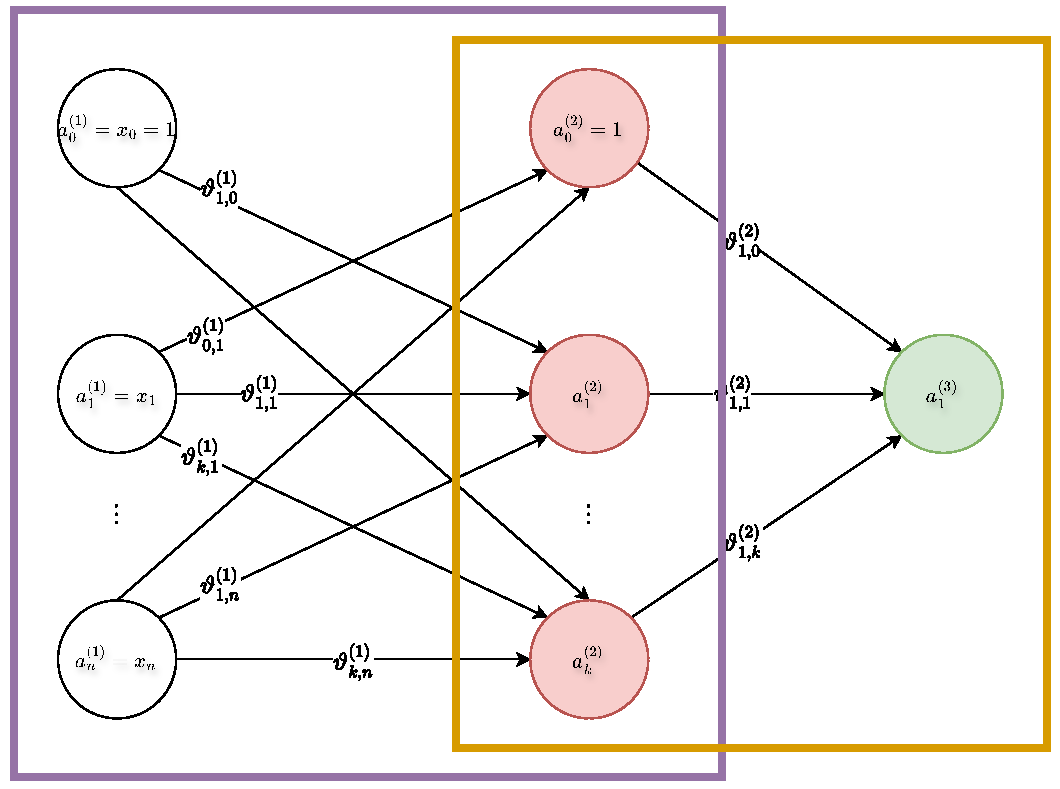
\includegraphics[width=0.75\linewidth]{images/NeuralNet2pdf}
	\caption{Un multilayer perceptron}
	\label{fig:nn_parts}
\end{figure}

Nella rete neurale fornita in figura \ref{fig:nn_parts}, individuiamo due parti.

\begin{itemize}
	\item La parte in viola della rete è dedicata alla \textbf{trasformazione degli input grezzi} in qualcosa di utile per il task. La trasformazione viene appresa in fase di training grazie alle etichette note dell'apprendimento supervisionato. In questo caso, permette di trasformare $x \to a^{(2)}$.
	
	\item La parte arancione invece è dedicata alla \textbf{classificazione} (tramite softmax, o regressore logistico nella classificazione binaria), prendendo come input i dati trasformati dal resto della rete, in questo caso $a^{(2)}$. Basta sostituire il softmax con un regressore lineare per usare la rete su task di regressione.
\end{itemize}


\section{Le funzioni di attivazione}
Le funzioni di attivazione devono essere derivabili per consentire il training della rete tramite algoritmo di discesa del gradiente e di backpropagation. Tra le funzioni più usate, abbiamo:

\begin{table}[ht]
	\centering
	\resizebox{\textwidth}{!}{%
		\begin{tabular}{lll}
			\hline
			\textbf{Nome} & \textbf{Equazione} & \textbf{Derivata} \\
			\hline
			Identità &
			$ f(x) = x $ &
			$ f'(x) = 1 $ \\[4pt]
			
			Gradino binario (Binary step) &
			$ f(x) =
			\begin{cases}
				0 & \text{per } x < 0,\\
				1 & \text{per } x \ge 0
			\end{cases} $ &
			$ f'(x) =
			\begin{cases}
				0 & \text{per } x \neq 0,\\
				? & \text{per } x = 0
			\end{cases} $ \\[8pt]
			
			Logistica (o Soft step) &
			$ f(x) = \dfrac{1}{1 + e^{-x}} $ &
			$ f'(x) = f(x)\bigl(1 - f(x)\bigr) $ \\[8pt]
			
			TanH &
			$ f(x) = \tanh(x) = \dfrac{2}{1 + e^{-2x}} - 1 $ &
			$ f'(x) = 1 - f(x)^2 $ \\[8pt]
			
			ArcTan &
			$ f(x) = \tan^{-1}(x) $ &
			$ f'(x) = \dfrac{1}{x^2 + 1} $ \\[8pt]
			
			Unità lineare rettificata (ReLU) &
			$ f(x) =
			\begin{cases}
				0 & \text{per } x < 0,\\
				x & \text{per } x \ge 0
			\end{cases} $ &
			$ f'(x) =
			\begin{cases}
				0 & \text{per } x < 0,\\
				1 & \text{per } x \ge 0
			\end{cases} $ \\[8pt]
			
			Unità lineare rettificata parametrica (PReLU) &
			$ f(x) =
			\begin{cases}
				\alpha x & \text{per } x < 0,\\
				x        & \text{per } x \ge 0
			\end{cases} $ &
			$ f'(x) =
			\begin{cases}
				\alpha & \text{per } x < 0,\\
				1      & \text{per } x \ge 0
			\end{cases} $ \\[8pt]
			
			Unità lineare esponenziale (ELU) &
			$ f(x) =
			\begin{cases}
				\alpha\left(e^{x} - 1\right) & \text{per } x < 0,\\
				x                            & \text{per } x \ge 0
			\end{cases} $ &
			$ f'(x) =
			\begin{cases}
				f(x) + \alpha & \text{per } x < 0,\\
				1             & \text{per } x \ge 0
			\end{cases} $ \\[8pt]
			
			SoftPlus &
			$ f(x) = \log_e\!\bigl(1 + e^{x}\bigr) $ &
			$ f'(x) = \dfrac{1}{1 + e^{-x}} $ \\[4pt]
			\hline
		\end{tabular}%
	}
\end{table}

Riportiamo alcuni dei plotting delle funzioni di attivazione e le loro derivate. 

\begin{figure}[htp]
	\centering
	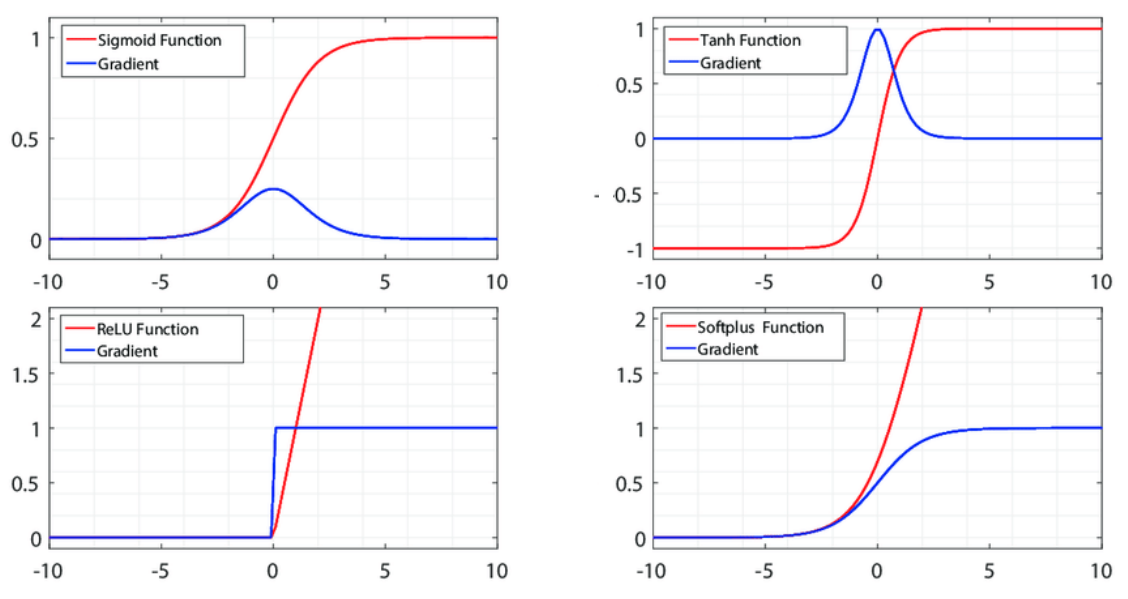
\includegraphics[width=0.8\linewidth]{images/activation-functions}
\end{figure}

\section{Il teorema di approssimazione universale per le reti neurali}\label{sec:teorema_approssimazione_universale}

\begin{quote}
	Il \textit{Teorema di Approssimazione Universale} afferma che una rete neurale feed-forward\footnote{Per feed-forward si intende una rete neurale in cui ogni layer riceve input esclusivamente dal layer precedente e lo trasmette a quello successivo, senza cicli o connessioni ricorrenti.} con un solo \emph{hidden layer}, dotata di un numero finito ma sufficientemente grande di neuroni e di una funzione di attivazione non lineare (ad esempio sigmoide o tangente iperbolica), è in grado di approssimare qualunque funzione continua definita su un insieme compatto $K \subset \mathbb{R}^n$, con errore arbitrariamente piccolo.
\end{quote}

\noindent
Più formalmente, data una funzione continua
\[
f : K \subset \mathbb{R}^n \to \mathbb{R}
\]
e fissato un qualunque $\varepsilon > 0$, esiste una rete neurale con un solo strato nascosto tale che
\[
\sup_{x \in K} | f(x) - \hat{f}(x) | < \varepsilon,
\]
dove $\hat{f}(x)$ rappresenta la funzione implementata dalla rete neurale.

\paragraph{Interpretazione.}
Il risultato implica che una rete neurale con un solo hidden layer possiede una capacità espressiva teoricamente universale: non è limitata, in linea di principio, nel tipo di funzione che può rappresentare. La limitazione non è dunque strutturale, ma riguarda piuttosto il processo di apprendimento dei parametri e la quantità di neuroni necessari per ottenere una buona approssimazione.

\paragraph{Esempio.}
Consideriamo la funzione
\[
f(x) = \sin(x), \qquad x \in [0, 2\pi].
\]
Una rete neurale con attivazioni sigmoidi può combinare molte sigmoidi traslate e scalate per costruire una curva che approssima la sinusoide con errore arbitrariamente piccolo. Aumentando il numero di neuroni nello strato nascosto, la rete riesce a rappresentare dettagli sempre più fini dell’andamento della funzione.

\paragraph{Limiti del teorema.}
È importante sottolineare che il teorema non fornisce un metodo costruttivo per determinare i parametri della rete, né garantisce che un algoritmo di ottimizzazione (come la discesa del gradiente) riesca effettivamente a trovare la configurazione che realizza l’approssimazione desiderata. Inoltre, il teorema non dice nulla sulla capacità di generalizzazione del modello né fornisce un limite superiore sul numero di neuroni necessari, che potrebbe essere molto elevato. In pratica, una rete con un solo hidden layer potrebbe richiedere un numero enorme di neuroni per rappresentare funzioni complesse, risultando inefficiente e potenzialmente soggetta a overfitting.

Questo risultato teorico fornisce quindi una motivazione concettuale all’uso delle reti \emph{deep}: l’introduzione di più strati nascosti consente spesso di rappresentare le stesse funzioni in modo più compatto ed efficiente.



\section{Training e inferenza di una rete neurale}
\begin{figure}[tbph]
	\centering
	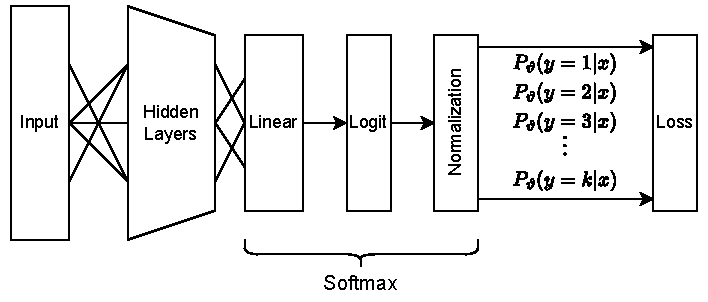
\includegraphics[width=1\linewidth]{images/neural-net}
	\caption{Struttura tipica di una rete neurale per la classificazione.}
\end{figure}

Durante la fase di training, il nostro obiettivo è quello di stabilire i migliori parametri per il nostro modello sui dati di training. Usiamo quindi la Loss function e la nostra procedura di training. Usiamo poi il modello con i parametri ottenuti per fare inferenza su nuovi dati, e osservare le performance del modello.


\subsection{Funzione di costo}
Definiamo la nostra funzione di costo.

$$
J(\vartheta) = -\frac{1}{m} \sum_{i=1}^{m} \underbrace{\sum_{c=1}^{k}\mathbf{1}\{y^{(i)} = c\} \log(h_\vartheta^{(c)}(x^{(i)}))}_\text{Cross Entropy Loss Function}
$$

\noindent 
in cui
\begin{itemize}
	\item $m$ = numero di esempi nel dataset
	\item $k$ = numero di classi
	\item $(x^{(i)})$ = $i$-esimo input
	\item $(y^{(i)})$ = etichetta (classe corretta) dell’$i$-esimo esempio
	\item $(\mathbf{1}(y^{(i)} = c))$ = funzione indicatrice: vale 1 se l’esempio ($i$) appartiene alla classe ($c$), altrimenti 0
	\item $(h_\theta^{(c)}(x^{(i)}))$ = output della rete (probabilità predetta) per la classe ($c$) sull’esempio ($i$)
\end{itemize}

\noindent
Il nostro obiettivo è quello di trovare $\hat{\vartheta}$, ossia i valori dei parametri $\vartheta$, tali che
$$
\hat\vartheta = \min(J(\vartheta))
$$


\subsection{Chain Rule}
Considerando le reti neurali come delle funzioni composte, o annidate, è possibile usare la chain rule per le derivate di funzioni composte.

$$
\frac{\partial J(\vartheta)}{\partial\vartheta_{i,j}^{(l)}} \quad \forall j, i, l
$$ 


\subsection{Inizializzazione dei parametri}
L'inizializzazione dei parametri avviene con numeri casuali molto piccoli $\in [-\varepsilon, +\varepsilon]$. I parametri dei nodi che dipendono dallo stesso nodo, devono essere diversi tra loro, effettuando quella che è nota come \textbf{symmetry breaking}.

In pratica, si assegna a neuroni dello stesso layer inizializzazioni diverse, così che non producano le stesse attivazioni e non ricevano gradienti identici. 

\paragraph{Perché è importante?} Senza symmetry breaking, tutti i neuroni apprenderebbero la stessa funzione attraverso gli stessi gradienti durante la backpropagation, rendendo inefficace l'avere più neuroni nello stesso layer. Questo annullerebbe i benefici della profondità e della larghezza della rete, poiché ogni neurone comporterebbe solo una moltiplicazione ridondante dei pesi identici.

\subsection{Reti neurali per regressione}
Usiamo come Loss function l'errore quadratico medio (MSE). Ogni output sarà un regressore lineare, e la Loss function valuterà gli output di tutti i regressori.
\begin{figure}[tbph]
	\centering
	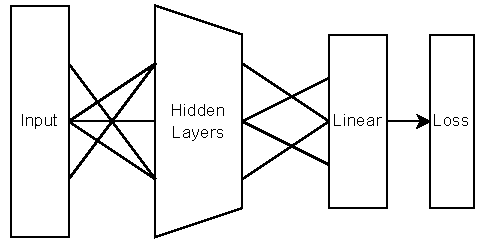
\includegraphics[width=0.8\linewidth]{images/linear-reg-neuralnet}
\end{figure}


\section{Overfitting e Underfitting nelle reti neurali}
\paragraph{Underfitting.} Le reti neurali più piccole, su dati molto complessi, sono soggette ad underfitting. I pochi parametri non permettono di descrivere (o separare) i pattern complessi dei dati. Si riscontrano alti errori già in fase di training. Reti più semplici sono però più veloci da allenare.

\paragraph{Overfitting.} Le reti neurali più complesse, con tanti parametri, imparano meglio i dati in fase di training, minimizzando o addirittura azzerando la loss function. Il rischio è opposto: il modello diventa troppo specifico, e non riesce a generalizzare sui dati di testing, cadendo in overfitting. Diventa quindi necessario introdurre termini di regolarizzazione ($\lambda$) o cambiare modello. Modelli più vasti richiedono inoltre risorse computazionali più importanti.

\section{Caso studio: MLP}
Un MLP (Multi-Layer Perceptron) è una rete neurale feed-forward composta da più strati di neuroni, in cui ogni neurone di un layer è connesso a tutti i neuroni del layer successivo. Un esempio può essere visto in figura \ref{fig:mlp_nn}, in cui abbiamo un input layer, un hidden layer e un output layer. L’input layer riceve i dati in ingresso, l'hidden layer elabora le informazioni e l’output layer produce la predizione finale.

\subsection{Definizione del modello}
Consideriamo una rete neurale feed-forward completamente connessa, composta da un input layer, un hidden layer e un output layer. Indichiamo con $a^{(l)}$ il vettore delle attivazioni del layer $l$ e con $\Theta^{(l)}$ la matrice dei pesi che connette il layer $l-1$ al layer $l$. L’input della rete è $a^{(1)} = x$. Ogni neurone del layer successivo riceve in ingresso una combinazione lineare delle attivazioni del layer precedente; formalmente, per il generico layer $l$ definiamo

\[
z^{(l)} = a^{(l-1)} \Theta^{(l)},
\]

dove $z^{(l)}$ rappresenta il vettore delle combinazioni lineari. Il singolo neurone $j$ del layer $l$ è quindi dato da

\[
z_j^{(l)} = \sum_{i=1}^{n_{l-1}} a_i^{(l-1)} \theta_{i,j}^{(l)}.
\]

Applicando la funzione di attivazione $f$ elemento per elemento otteniamo

\[
a^{(l)} = f(z^{(l)}).
\]

Nel caso rappresentato in Figura~\ref{fig:mlp_nn}, ciascun neurone del layer nascosto riceve contributi da tutti i neuroni dell’input layer, mentre il neurone di output riceve contributi da tutte le unità del layer nascosto; la rete è quindi completamente connessa. L’output finale della rete è

\[
\hat{y} = a^{(L)}.
\]

\subsection{Funzione di costo}
Nel caso di classificazione multiclasse utilizziamo la Cross-Entropy Loss

\[
J(\vartheta) = -\frac{1}{m} \sum_{i=1}^{m} \sum_{c=1}^{k} \mathbf{1}\{y^{(i)} = c\} \log\big(h_\vartheta^{(c)}(x^{(i)})\big),
\]

dove $h_\vartheta(x^{(i)}) = a^{(L)}$ rappresenta l’output della rete per l’esempio $i$-esimo. Nel caso di regressione utilizziamo invece l’errore quadratico medio

\[
J(\vartheta) = \frac{1}{2m} \sum_{i=1}^{m} \|\hat{y}^{(i)} - y^{(i)}\|^2.
\]

L’obiettivo del training è determinare

\[
\hat{\vartheta} = \arg\min_{\vartheta} J(\vartheta).
\]

\subsection{Backpropagation}
Poiché la rete neurale è una composizione di funzioni, il calcolo dei gradienti avviene tramite la chain rule. Definiamo il termine di errore del layer $l$ come

\[
\delta^{(l)} = \frac{\partial J}{\partial z^{(l)}}.
\]

Per l’output layer si ottiene

\[
\delta^{(L)} = a^{(L)} - y.
\]

Per un generico layer interno vale invece

\[
\delta^{(l)} = \left( \delta^{(l+1)} (\Theta^{(l+1)})^\top \right) \odot f'(z^{(l)}),
\]

dove $\odot$ indica il prodotto elemento per elemento. Il gradiente rispetto ai pesi del layer $l$ risulta

\[
\frac{\partial J}{\partial \Theta^{(l)}} = (a^{(l-1)})^\top \delta^{(l)}.
\]

\subsection{Aggiornamento dei parametri}
Una volta calcolati i gradienti, i parametri vengono aggiornati tramite discesa del gradiente secondo la regola

\[
\Theta^{(l)} \leftarrow \Theta^{(l)} - \alpha \frac{\partial J}{\partial \Theta^{(l)}},
\]

dove $\alpha > 0$ rappresenta il learning rate. Il processo viene ripetuto iterativamente fino alla convergenza, ossia fino a quando la funzione di costo non varia in modo significativo oppure viene raggiunto un numero massimo di iterazioni.

\subsection*{Interpretazione}
Un MLP realizza una sequenza di trasformazioni lineari seguite da funzioni di attivazione non lineari. Le trasformazioni lineari combinano le informazioni provenienti dal layer precedente, mentre le non linearità permettono alla rete di rappresentare funzioni complesse e di modellare relazioni non lineari tra input e output. Il training consiste nella regolazione iterativa dei pesi $\Theta^{(l)}$ in modo da minimizzare la funzione di costo; grazie alla composizione di più layer, la rete è in grado di apprendere rappresentazioni interne progressivamente più astratte dei dati in ingresso.

\section*{Riferimenti}
I riferimenti per questo capitolo includono:
\begin{itemize}
	\item Materiale visto a lezione.
	\item Teorema di approssimazione universale per le reti neurali \ref{sec:teorema_approssimazione_universale} dal libro \citetitle{Goodfellow-et-al-2016} \cite{Goodfellow-et-al-2016}, sezione 6.4.1.
	\item Caso studio MLP scritto da Paolo Volpini, \url{https://github.com/paolovolpini}.
\end{itemize}